\section{QuickSort}

\subsection{Algemeen}

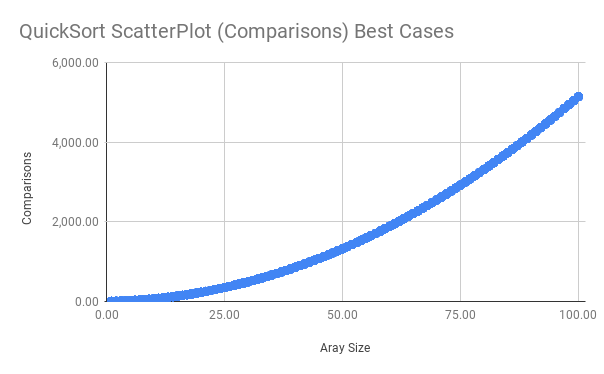
\includegraphics[scale=0.3]{sections/media/QS_C_BC}
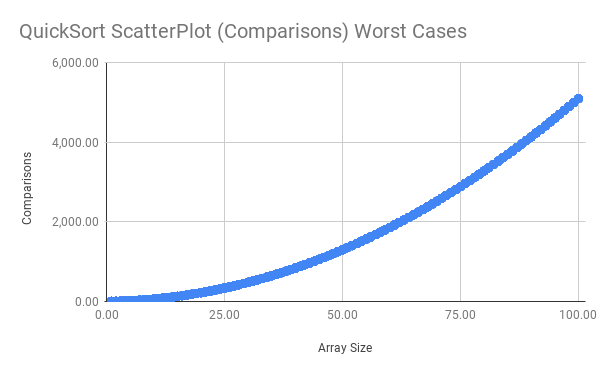
\includegraphics[scale=0.3]{sections/media/QS_C_WC}
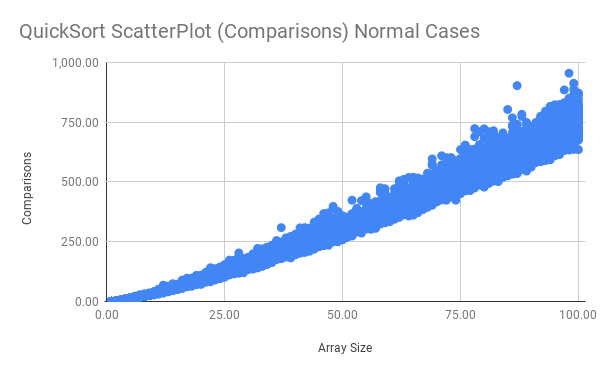
\includegraphics[scale=0.6]{sections/media/QS_C_NC}

QuickSort is een divide-and-conquer algoritme. Het werkt door een \textit{pivot} te kiezen uit de array en het array daar te partitioneren in twee sub-arrays gebaseerd op of dat het element groter of kleiner is als de \textit{pivot}, de twee sub-arrays worden dan recursief gesorteerd door hetzelfde algoritme.

Theoretisch gezien is QuickSort een \(\sim 1,39nlog(n)\) algoritme.

We kunnen zien aan de grafiek dat in de normale gevallen, net zoals InsertionSort, dat er een grote verspreiding is in de vergelijkingen van het algoritme. Omdat het best-case scenario voor QuickSort niet de echt best-case scenario is, krijgen we niet de theoretisch berekende \(nlog(n)\) vergelijkingen. Hetzelfe voor het worst-case scenario, we krijgen niet de theoretisch berekende \(n^2\).

\newpage

\subsection{Doubling Ratio}

\begin{table}[hp!]
    \centering
    \begin{tabular} {c | c | c}
        \textbf{AS(N)} & \textbf{MT(N)} & \textbf{MR(N)} \\
        \hline
        20 000 & 1.75 ms & 1.94 \\
        \hline
        40 000 & 3.85 ms & 2.20 \\
        \hline
        80 000 & 8.60 ms & 2.23 \\
        \hline
        160 000 & 20.70 ms & 2.41 \\
        \hline
        320 000 & 38.35 ms & 1.85 \\
        \hline
        640 000 & 88.10 ms & 2.30 \\
    \end{tabular}
    \caption{QuickSort Doubling Ratio Measurements}
\end{table}


Het doubling ratio experiment levert de bovenstaande tabel op. We verwachten dat het doubling ratio 2 nadert want, \(T(2)=2\log_2(2)=2\) en als N 2 keer zo groot was zou \(T(N)\) ook ongeveer 2 moeten zijn. We zien dan ook dat het doubling ratio snel deze theoretische limiet nadert.

\begin{table}[hp!]
    \centering
    \begin{tabular} {c | c | c | c | c}
        \textbf{AS(N)} & \textbf{PT(N)} & \textbf{PR(N)} & \textbf{MT(N)} & \textbf{MR(N)} \\
        \hline
        1 280 000 & 176.20 ms & 2.00 & 250.70 ms & 2.85 \\
        \hline
        2 560 000 & 352.40 ms & 2.00 & 561.30 ms & 2.24 \\
        \hline
        5 120 000 & 704.80 ms & 2.00 & 1 325.20 ms & 2.36 \\
    \end{tabular}
    \caption{QuickSort Doubling Ratio Predictions}
\end{table}


Voor de voorspelling is als doubling ratio 2 genomen zoals hierboven besproken. We zien uit de tabbel dat de voorspelling zich ongeveer richten met de metingen. Als we nu een voorspelling maken voor een problem size N die 8 keer groter is aals onze grootste meeting, dan bekomen we: \(1325,20*2^8=338995,2\) of \(\sim 338\) seconden. Dit is trouwens veel sneller dan bijde InsertionSort en SelectionSort.
